\section{Durchführung}
\label{sec:Durchführung}

\subsection{Messvorrichtung}
Zur Vermessung der elastischen Stäbe wird die Apperatur in \autoref{fig:messung} verwendet. In dieser lässt sich der Stab entweder beidseitig oder auch
einseitig einspannen. Auf einer Skala sind verschiebare Messuhren angebracht, die die Höhenauslenkung sehr genau messen können. Mithilfe eines Halters kann 
ein Gewicht am Ende des einseitig angespannten Stabes oder in der Mitte eines beidseitig angespanntes Stabes angebracht werden. Da nicht ausgeschlossen werden kann,
dass die Stäbe nicht schon etwas verbogen sind, ist darauf zu achten die Messuhren vor jeder Messung einmal ohne anhängendes Gewicht zu nullen.
\begin{figure}[H]
    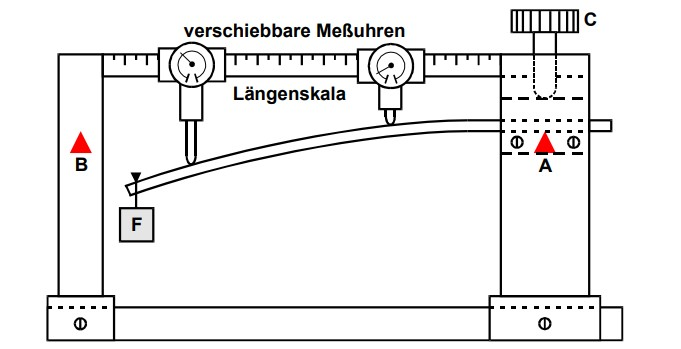
\includegraphics[width=\linewidth]{img/abb5.jpg}
    \caption{Apperatur zur Vermessung elastischer Stäbe.\cite{V103}}
    \label{fig:messung}
\end{figure}

\subsection{Versuchsablauf}
Zu Beginn werden jeweils ein runder und ein eckiger Stab gewogen und vermessen. Die Masse der Anhängelast und der Halterung wird ebenfalls bestimmt.
Der zu vermessende Stab wird einseitig in die Vorrichtung eingespannt. Für die einseitige Einhängung wird eine Anhängelast von $m = \SI{500}{g}$ gewählt. 
Bei der Wahl der Anhängelast ist es nur wichtig, dass das Gewicht nicht den Boden berührt. Es werden nun 20-25 Messwerte entlang der Skala aufgenommen. 
Bei jeder Messung wird zuerst die Auslenkung auf 0 gesetzt, bevor die Last angehangen wird. Dieser Vorgang wird für beide Stäbe durchgeführt.
\\
\\
Anschließend wird der zu vermessende Stab beidseitig eingespannt. Hier werden mittig $m = \SI{1000}{g}$ angehangen. Analog werden 25-30 Messwerte über die
volle Skala verteilt aufgenommen. Der Vorgang wird ebenfalls für beide Stäbe durchgeführt.